\documentclass[12pt]{article}
\usepackage{fancyhdr}
\usepackage{lastpage}
\usepackage{geometry}
\usepackage{amsmath}
\usepackage{setspace}
\usepackage{graphicx}
\usepackage{caption}
\geometry{a4paper,scale=0.8}
\pagestyle{plain}
\renewcommand{\headrulewidth}{0.4pt}
\renewcommand{\footrulewidth}{0.4pt}
\setlength{\baselineskip}{23pt}


\begin{document}
	\thispagestyle{plain}
	\noindent \Large \textbf{Multi-Factor stock pitching model using ML}\\ \\
	\noindent Fu, Sun, Wang BY, Wang PY and Zhuang (2019)\\
	\noindent \normalsize \textit{Singapore Management University, Singapore}\\ \\
	\noindent July 2019
	
\section{Abstract} % Numbered section
	
	text..
	
\section{Introduction} % Numbered section
     text..

		
\section{Data}
text..


\section{Methodology \& Research Design}
text..

\newpage
\section{Backtest Results}

In this section, we construct a simple investment strategy based on the previous SVM or SGD model's prediction. The logic of this strategy can be stated as: we select 100 stocks with the highest possibility of positive return in the following month under SVM model prediction and adopted a equal weight among all the stocks. The Net Asset Value (NAV) of the portfolio can be visualized as the cumulative excess return line in the figure below.\\ \\

\noindent And we evaluate each portfolio's performance based on three indicators:
	\begin{itemize}
		\item Annual excess return: Calculated by $12*\mu$, where $\mu$ is the average excess return of one year.
		\item Anuual excess volatility: Calculated by $\sqrt{12 * \sigma^2}$, where $\sigma^2$ is the annual variance of whole year excess return 
		\item Information Ratio (IR): Calculated by $\frac{\textnormal{Anuual excess return}}{\textnormal{Annual excess volatility}}$ , and it can be translated as the premium for portfolio taking each unit of active risk. So the bigger IR is, the better portfolio perform.
	\end{itemize}

\begin{figure}[h]
	\centering
	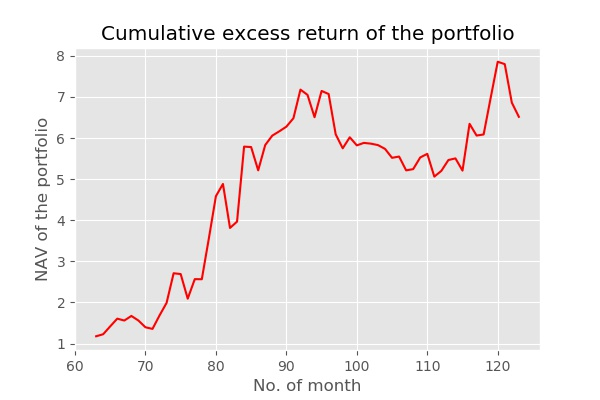
\includegraphics[width=0.6\linewidth]{pic//NAV_SVM.jpg}
	\caption*{Figure 01: Portfolio based on SVM}
	\label{fig:label}
\end{figure}

\begin{figure}[h]
	\centering
	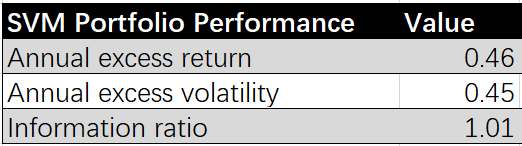
\includegraphics[width=0.6\linewidth]{pic//SVM_Performance.png}
	\caption*{Table 01: SVM Portfolio performance}
	\label{fig:label}
\end{figure}
\newpage
\begin{figure}[h]
\centering
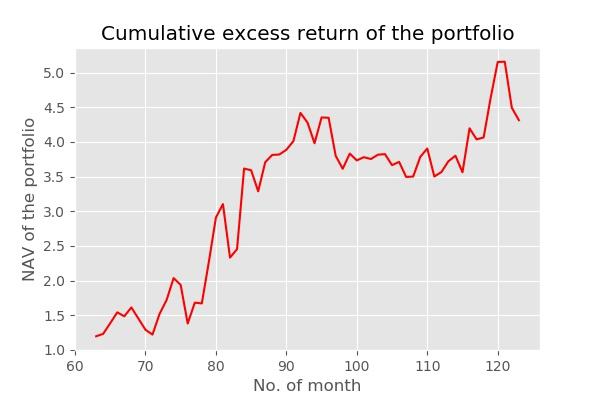
\includegraphics[width=0.6\linewidth]{pic//NAV_SGD.jpg}
\caption*{Figure 02: Portfolio based on SGD}
\label{fig:label}
\end{figure}

\begin{figure}[h]
	\centering
	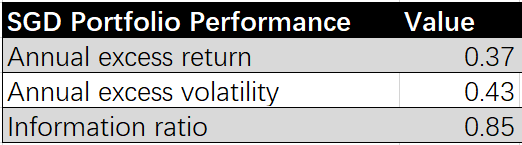
\includegraphics[width=0.6\linewidth]{pic//SGD_Performance.png}
	\caption*{Table 02: SGD Portfolio performance}
	\label{fig:label}
\end{figure}



\section{Conclusion} % Numbered section

text..



\end{document}
